\section{Implementation overview}

The solution is presented as an open-source library, that provides the major part of genetic algorithm implementation, which can be shared between different application. Base algorithm consist of a pipeline separated by three stages: selection, crossover and mutation, which evolves the population of individuals, increasing average level of adjustment and finding the best individual according to provided fitness function; preimplemented most popular strategies of genetic selection, crossover and mutation, with possibility of extanding with the additional ones for specific reasons and a set of platforms which allow to run the pipeline in a different ways, best suited for existing hardware. The library is supplied with key features, basing on the concepts described earlier, wrapping all the components into sufficient framework.

\subsection{Technology stack}

\subsubsection{Scala programming language}

Scala is a modern multi-paradigm programming language designed to express common programming patterns in a concise, elegant, and type-safe way. Its name stands for "scalable language." The language is so named because it was designed to grow with the demands of its users. It can be applied to a wide range of programming tasks, from writing small scripts to building large systems.
Scala is easy to get into. It runs on the standard Java platform and interoperates seamlessly with all Java libraries. It's quite a good language for writing scripts that pull together Java components. But it can apply its strengths even more when used for building large systems and frameworks of reusable components. \cite{programming_in_scala}

Technically, Scala is a blend of object-oriented and functional programming concepts in a statically typed language. The fusion of object-oriented and functional programming shows up in many different aspects of Scala; it is probably more pervasive than in any other widely used language. The two programming styles have complementary strengths when it comes to scalability. Scala's functional programming constructs make it easy to build interesting things quickly from simple parts. Its object-oriented constructs make it easy to structure larger systems and adapt them to new demands. The combination of both styles in ScaalMatei Zaharia, “Spark: Cluster Computing with Working Sets
 makes it possible to express new kinds of programming patterns and component abstractions. It also leads to a legible and concise programming style \cite{programming_in_scala}

% May be expanded with definitions from books

Due to its programming style and variety of features Scala serves a great tool for developing this library. A combination of paradigms is extremely usefull in this case and was crutial during selection of programming language. Both of the programming styles were heavily used in order to gain the best possible result:
\begin{itemize}
\item
Object-oriented style

Scala is an object-oriented language in pure form: every value is an object and every operation is a method call. \cite{programming_in_scala} It provides modularity and maintainability: all application is split into a self-sufficient containers, which store the relevant data and provide available operations, that may be performed on its data. These containers may be used as the assembling parts for another container, passed as function parameter and returned as function result. Such approach allows to keep track of the growing codebase, alligning its components into domain hierarchies and letting its parts to comunicate with one another.

\item
Functional style

Functional programming provides expressiveness, composability and conciseness. Building the library with mathematical-like functions makes it more understandable, replacing the mutable state from the application. As the result, it becomes clear, unequivocal and may be safely used in multi-thread environment. One of the most important assets, which comes from functional programming, is scalability. A well constructed application may easily be enlarged for user needs to handle a growing amount of work; it is more adaptive to the changing needs and the performance of such system improves proportionally to the additional hardware.

\end{itemize} 

 \textbf{Parallel collections}

 Encouraging usage of immutable objects, from version 2.8 Scala provides new collection API, which contains parallel collections package as part of it. Parallel collections were included in the Scala standard library in an effort to facilitate parallel programming by sparing users from low-level parallelization details, meanwhile providing them with a familiar and simple high-level abstraction. The idea is simple– collections are a well-understood and frequently-used programming abstraction. And given their regularity, they’re able to be efficiently parallelized, transparently. By allowing a user to “swap out” sequential collections for ones that are operated on in parallel, Scala’s parallel collections take a large step forward in enabling parallelism to be easily brought into more code. \cite{scala_parallel_collections_overview}

 How parallel collections are built?
 What may be acquired with scala parallel collections?


\subsubsection{Apache Spark}

Apache Spark is a high-performance, general-purpose distributed computing system that has become the most active Apache open source project, with more than 1,000 active contributors. Spark enables users to process large quantities of data, beyond what can fit on a single machine, with a high-level, relatively easy-to-use API. Spark’s design and interface are unique, and it is one of the fastest systems of its kind. Uniquely, Spark allows to write the logic of data transformations and machine learning algorithms in a way that is parallelizable, but relatively system agnostic. So it is often possible to write computations that are fast for distributed storage systems of varying kind and size.

On the generality side, Spark is designed to cover a wide range of workloads that previously required separate distributed systems, including batch applications, iterative algorithms, interactive queries, and streaming. By supporting these workloads in the same engine, Spark makes it easy and inexpensive to combine different processing types, which is often necessary in production data analysis pipelines.\cite{learning_spark}

Spark can run over a variety of cluster managers to access the machines in a cluster. The easiest way is to run Spark by iteself on a set of machines. For this purpose Spark comes with built-in Standalone mode. Spark’s Standalone manager offers a simple way to run applications on a cluster. It consists of a master and multiple workers, each with a configured amount of memory and CPU cores. When application is submited, one can choose how much memory its executors will use, as well as the total number of cores across all executors.

Spark Core contains the basic functionality of Spark, including components for task scheduling, memory management, fault recovery, interacting with storage systems, and more. Spark Core is also home to the API that defines resilient distributed data‐sets (RDDs), which are Spark’s main programming abstraction. RDDs represent a collection of items distributed across many compute nodes that can be manipulated in parallel. Spark Core provides many APIs for building and manipulating these collections. RDDs offer two types of operations: transformations and actions. Transformations construct a new RDD from a previous one. For example, one common transformation is filtering data that matches a predicate. Actions are operations, which produce different result than the transformation, like collecting the elements into a local collection on master node or counting the number of elements in RDD. Transformations and actions are different because of the way Spark computes RDDs. Although new RDDs can be defined in any time, Spark computes them only in a lazy fashion — that is, the first time they are used in an action. The transformations, on the other hand, are scheduled to a DAG (directed acyclic graph) of computations. This approach has a lot of advantages, among them: effective fault tollerance and ability to make a lot of optimization decisions before actually running operations. This would not be possible if it executed computations as soon as it got it.

In distributed mode, Spark uses a master/slave architecture with one central coordinator and many distributed workers. The central coordinator is called the driver. The driver communicates with a potentially large number of distributed workers called executors. The driver runs in its own Java process and each executor is a separate Java process. A driver and its executors are together termed a Spark application. Then a Spark application is launched on a set of machines using early described cluster manager.

\begin{figure}
\centering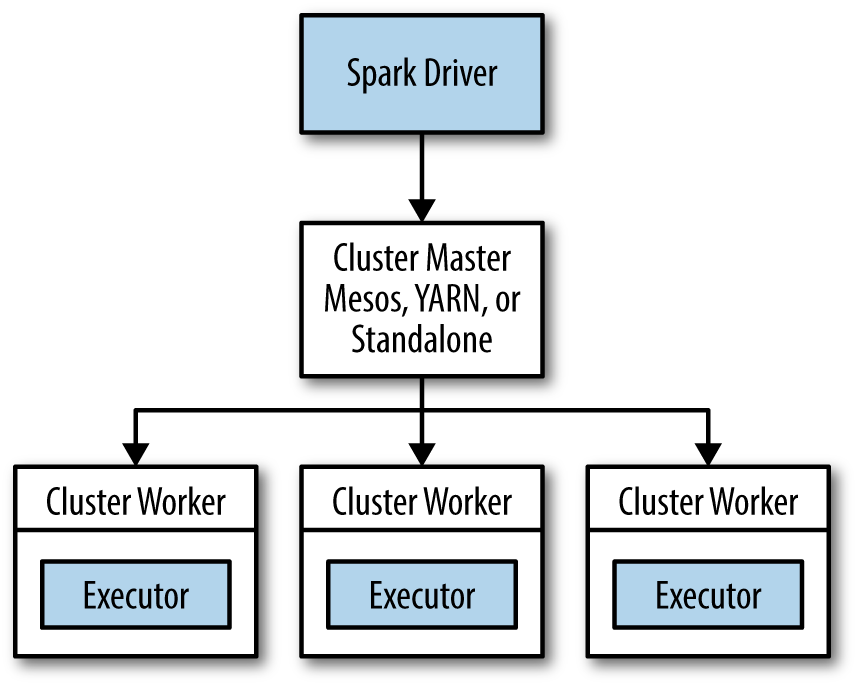
\includegraphics[width=.6\textwidth]{img/spark-runtime-split}
\caption{ The components of a distributed Spark application \cite{learning_spark}.}  \label{img:spark-components}
\end{figure}

This architectures allows to distribute the data between different executor nodes and perform operations on it locally until the shuffling is needed. Only then the data is shared between different nodes and the network communication is handled. In a distributed program, communication is very expensive, so laying out data to minimize network traffic can greatly improve performance. Much like how a single-node program needs to choose the right data structure for a collection of records, Spark programs can choose to control their RDDs’ partitioning to reduce communication.

In order to be able to transforms large sets of data without redundant recomputation Spark provides data persistence. When the Spark is asked to persist an RDD, the nodes that compute the RDD store their partitions. Spark has many levels of persistence to choose from based on what the goals are. The list of storage levels with performance comparison may is shown on \ref{img:spark_persistence_levels}. Combining different persistence modes, an executor can effectively share the data between its disk and RAM.

\begin{figure}
\centering 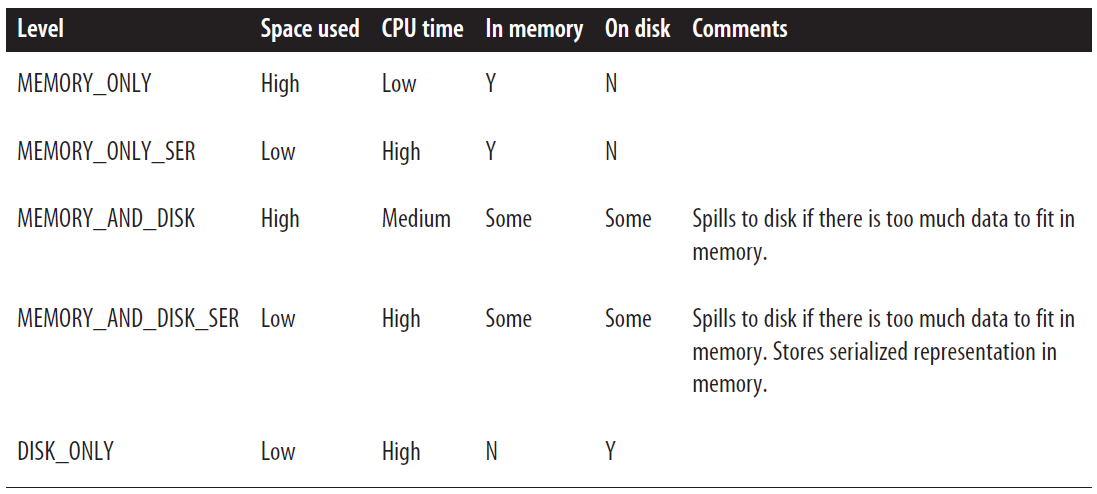
\includegraphics[width=.6\textwidth]{img/spark_persistence_levels}
\caption{ Persistence levels from org.apache.spark.storage.StorageLevel and
pyspark.StorageLevel \cite{learning_spark}.}\label{img:spark_persistence_levels}
\end{figure}



\subsubsection{Akka Streams}


Akka Streams is a library to process and transfer a sequence of elements using bounded buffer space. This latter property is what is ususally referred as boundedness and it is the defining feature of Akka Streams. Translated to everyday terms it is possible to express a chain of processing entities, each executing independently (and possibly concurrently) from the others while only buffering a limited number of elements at any given time. 

\begin{figure}
\centering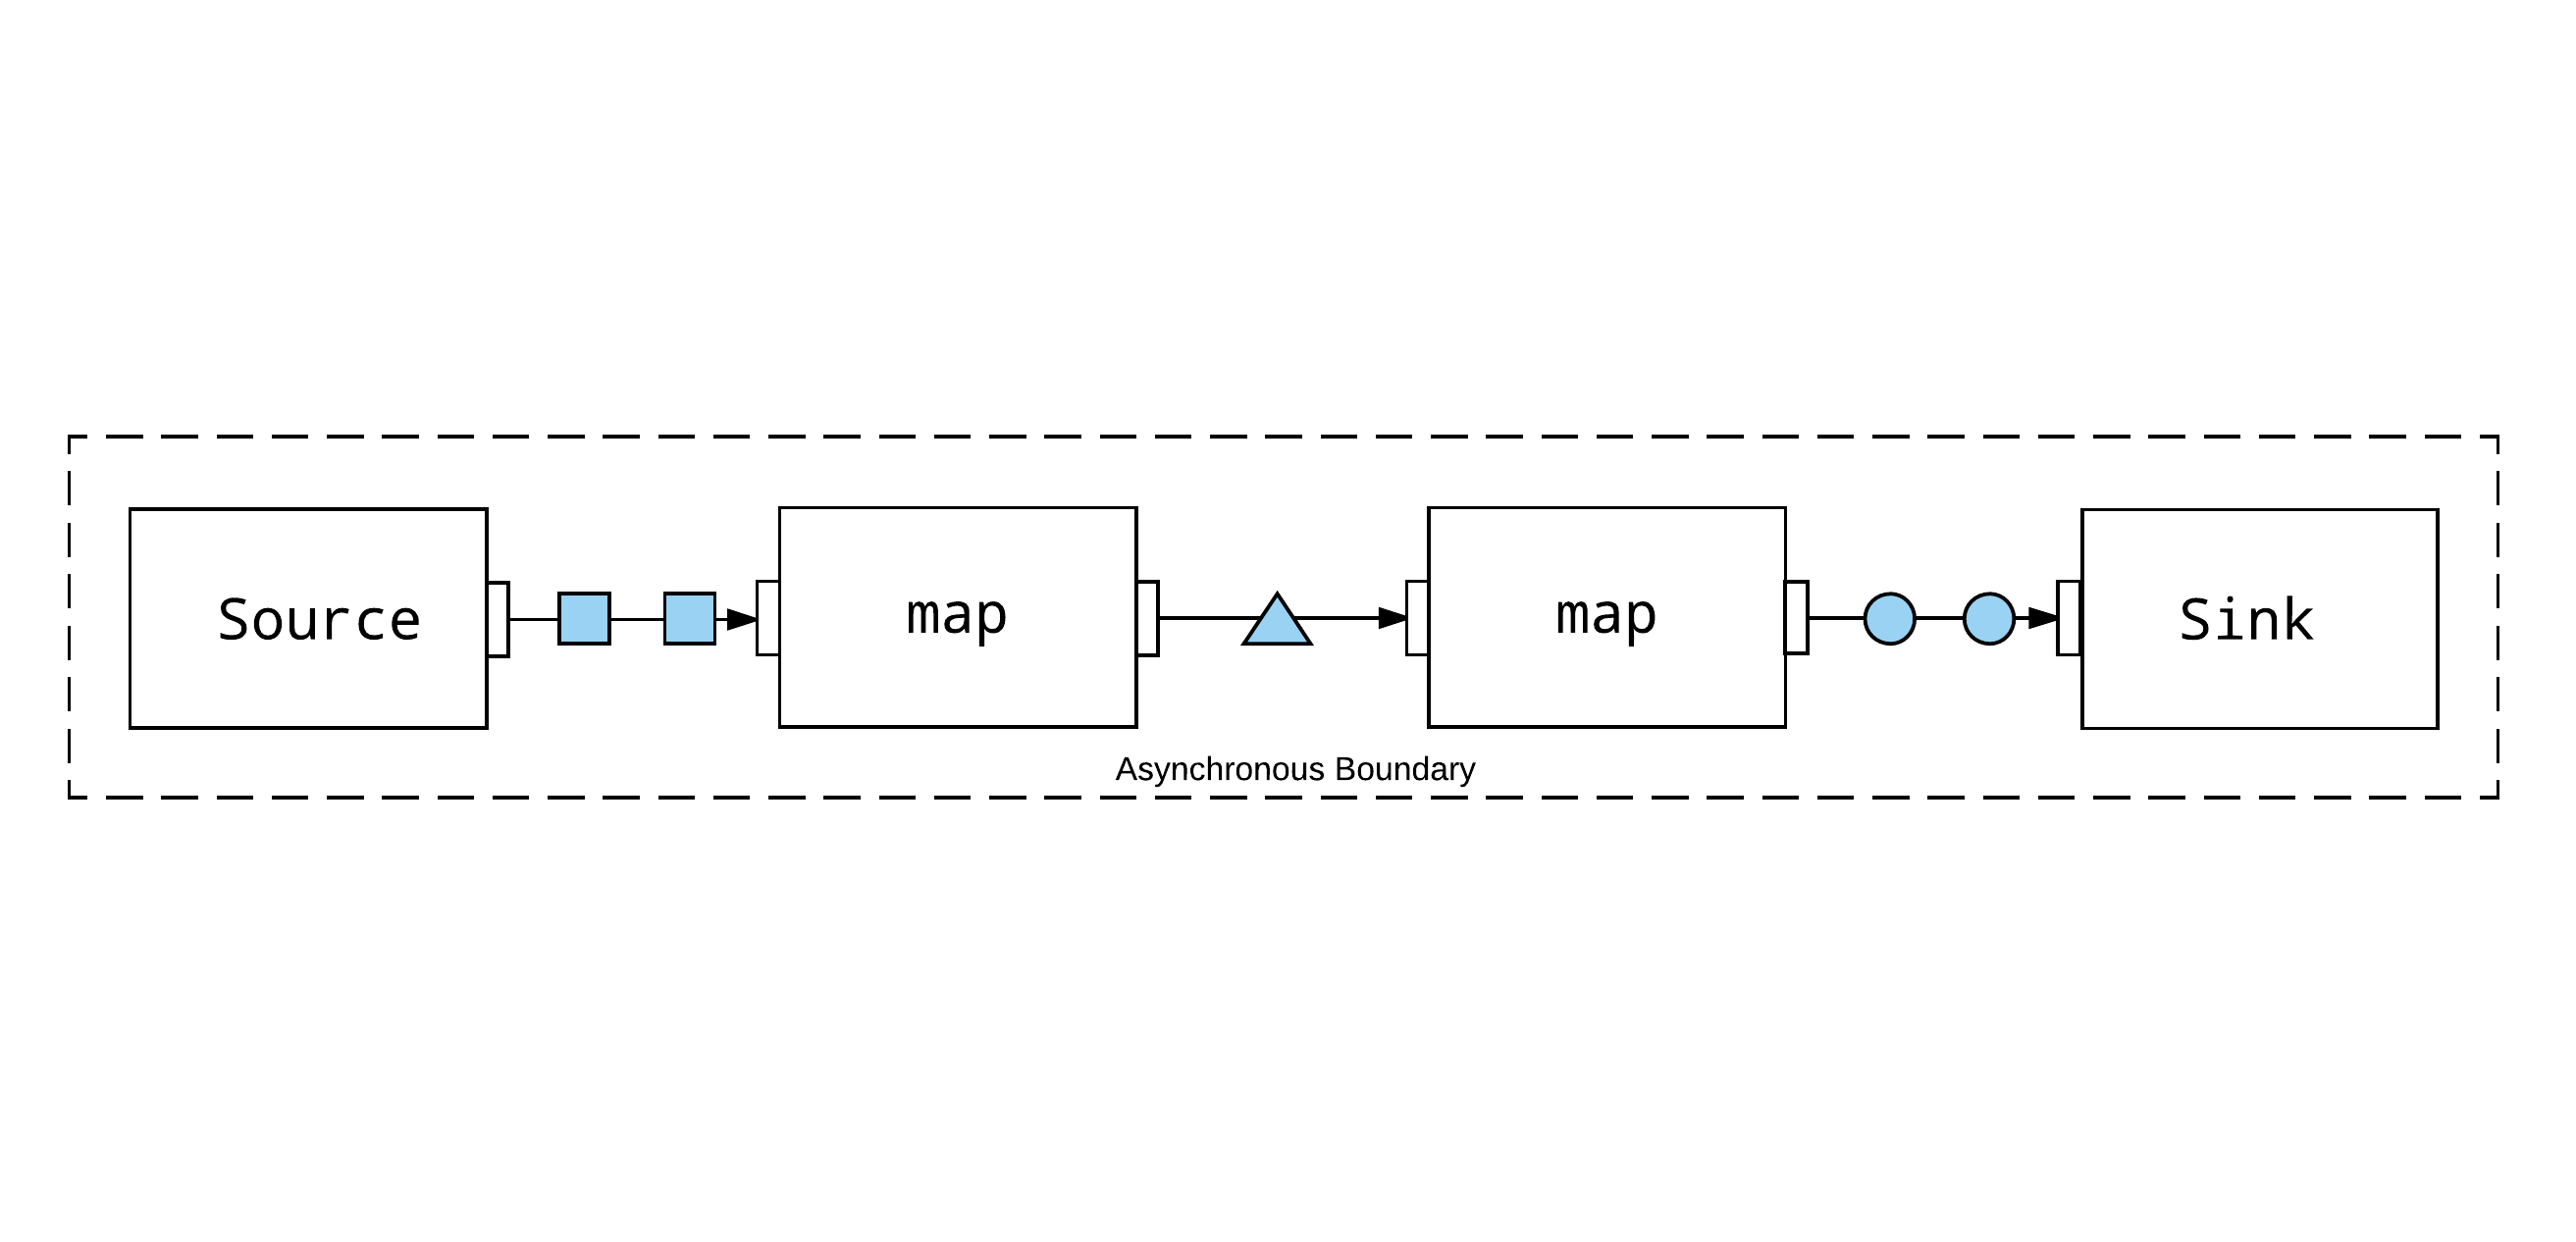
\includegraphics[width=.7\textwidth]{img/akka-streams-1}
\caption{A typical stream flow}\label{img:streams-1}
\end{figure}


\textit{ToDo: more info}


\subsection{Core components}

\textit{ToDo: add introduction}

\begin{itemize}

\item
Individual

An individual is a core component of genetic algorithm, often also reffered to as a \textit{genotype, chromosome \emph{or} a candidate}, which represents a candidate solution to a given problem. The number of individuals are evolved during the algorithm workflow, mixed and mutated in order to find the fittest one according to provided fitness function. This concept is purely abstract in the library, encoded as a generic type which may have an arbitrary representation defined by the users depending on their needs. 

In order to handle an individual through the process of evolution there should be defined a set of operators, where each encapsulates logic of some part of evolution procedure.   
\medbreak

\begin{itemize}
\item
Fitness

Fitness is a type class which represents a function of type \texttt{I => Double}, where \texttt{I} is type of individual. This function summarises how close a given design solution is to achieving the set aims. A ftness function must be devised for each problem to be solved, thus should be provided by the user and may not be preimplemented. Fitness function value is main criterion of future selection and is very important attribute of individual representation.

\textit{ToDo - how much does it cost}
\medbreak

\item
Join

Join is a type class, which represents a cross function of type \texttt{(I, I) => (I, I)}, where \texttt{I} is type of individual. This function defines how two instances of type \texttt{I} may be combined together to produce a new pair of \texttt{I}. It describes a crossover operation, due to which all the individuals from a population combined into pairs will be mixed during evolution process. An instance of the type class may be created from a single function of type \texttt{(I, I) => (I, I)}, as well as a function of type \texttt{(I, I) => I}. The latter case is suitable when identical function is used to compute both of result elements or in case of commutative operation. These cases were separated in order to enable memory allocation optimization by reusing the same product object to construct result pair.
\medbreak

\item
Modification

Modification is a type class, which represents a mutation function of type \texttt{I => I}, where \texttt{I} is type of individual. This operator is used to maintain generic diversity from one generation of a population to another. It is analogous to biological mutation. Mutation alters one or more gene values in a chromosome from its initial state, during which the solution may change entirely from the former shape. Because of its loose representation (even identity function may be considered as modification) it is important to provide a set of laws, which will distinguish a modification, which actually brings a diversity into the population. A \textit{lawfull} modification function is one, which holds following properties:

\begin{enumerate}
\item
A modified instance does not equal to original one (\textit{e.i modification function does not equal to identity function}) \ref{listing:mod1}

\begin{listing}
\begin{minted}{python}
	modify(i) != i
\end{minted}
\caption{The first laws of Modification instance} \label{listing:mod1}
\end{listing}

\item
After a certain number of modification the same input produces different outputs (\textit{ e.i. modification function is randomized or depends on outer variables}) \ref{listing:mod2}

\begin{listing}
\begin{minted}{python}
	def modify5(i: I) = modify(modify(modify(modify(modify(i)))))
	modify5(i) != modify5(i)
\end{minted}
\caption{The second laws of Modification instance} \label{listing:mod2}
\end{listing}


\end{enumerate}
\medbreak

\item
Scheme

Scheme is a type class, which is responsible for a creation of new individual. This is additional function, which may be replaced by predefined initial population during the start of evolution process, but still offers more functionality and may be used when individuals are created randomly, from limitless iteratator, smaller collection, which should be cycled or even single instance of individual. This concept is implemented as a covariant class, so the scheme object of parent class may be replaced by the scheme object of child class. It allows to easily use this class with hierarchies, avoiding redundant code. 
\end{itemize} 

\smallskip \textit{Together this satisfies predefined functional requirement \ref{freq:generic}}

\medbreak

\item
Population

Population is a collecion of individuals, which holds them during single evolution step. Individuals are processed together and are viewed only as a part of population from the perspective of algorithm. During the evolution step the representation of population or holding type may be changed (e.g. after selection stage further processed population contains pair of individuals, which are meant to be mixed later).

From implementation perspective, population is a type alias to Scala vector collection. The choise of data structure was motivated by fast average performance and effectively constant random access time in particular.
\medbreak

\item
Evolution environment

Evolution environment is a component, which taking the set of options constructs endless evolution flow of given population and makes it ready to be run. It is a parent type to all implementations of different approaches in processing computations, which may be sequential or parallel, local or distributed. This concept is very important from the usage perspective as it devides the implementation of genetic algorithm from its usage, so the end user may even not be aware of the way how the evolution is performed. It is also the end point of all the dependent components, as there is no direct dependency to any of concrete implementation of evolution environment. This abstraction may be considered as high level representation of genetic algorithm itself. The list of concrete derivatives of this interace contains:
\begin{itemize}
\item[--]
Local environment

This type of environment presumes local evoluation of evolution flow. It is the richest environments in terms of possible configurations. The logic, behind the strategy of applying genetic operators and evaluating fitness values is decoupled from one another into instances of \texttt{EvolutionCompanion} and \texttt{FitnessEvaluator} classes respectively. For each of the strategies the are sequential and parallel versions, with additional fitness caching option for repetitive individuals within population. Any fitness evaluation strategy may combined with any possible technique of applying genetic operators, creating a number of possibilites ready for use.
\smallskip\textit{This satisfies predefined functional requirement \ref{freq:par}}
\medbreak

\item[--]
Asynchronous environment

Asynchronous environment delegates the function of fitness evaluation to another system, by sending non-blocking asynchronous calls for every element of the population. It may be extremely usefull for the problems with heavy fitness functions. This approach allows to compute fitness values on different machine or even cluster of machines, as well as using different low-level programming language or some specific optimization, with no need to switch the entire application to another platform. This type of environment also fits perfectly to cloud computing solutions, as fitness evaluation is entirely isolated from the rest of application. However, applying genetic operators in same way needs to send a lot more data over the network, which negates the benefits one can gain from this approach. For this reason, genetic operators are applied locally with any of the strategies described earlier.

\smallskip \textit{This satisfies predefined functional requirement \ref{freq:async}}

\medbreak

\item[--]
Distributed environment

Distributed environment is very different from the previous options. Here the evolution is performed on the population in terms Spark RDD, distributed over the cluster. This technique enables processing of very large population, since it is split between many executor nodes. Once the evolution step is done executors shuffle the data between each other in order to perform selection of individuals for the next population and continue working on the local values. It minimizes the network communication, which may be a bottle-neck in such applications. 

\smallskip\textit{This satisfies predefined functional requirement \ref{freq:distributed}}

\end{itemize}
\medbreak

\item
Evolution flow

Evolution flow represents the endless evolution process of given population. It is implemented as the reactive stream with one output, which may be plugged in into further part of pipeline or executed standalone. During running, evolution flow emits the instance of population once it is computed and starts working on the next one. Since it is a reactive stream, the process of evolution is continued during there is a demand from the downstream. For example, if the sink of pipeline needs to take only 50 first populations, no more than 50 will be computed. This technique allows to leave the variety of possible stop conditions to the end user, including number of elements pushed from the flow, total time, idle time since the last push or any predicate based on the last produced population(s). 

\smallskip\textit{This satisfies predefined functional requirements \ref{freq:stop}, \ref{freq:on-demand}, \ref{freq:best}}

\medbreak

\item Fitness caching

Fitness caching is implemented using decorator design pattern over the provided fitness function. It supports every fitness function provided by user, as it simply holds the record over the ranked individuals and returns stored result if it was encountered earlier. The data structure used for holding cached values is concurrent hash trie. It guarantees consistency in multithreaded environment, enabling safe usage with parallel workflows. From the performance side, concurrent hash tries allow to lookup element in logarithmic time, with costant snapshot time \cite{hash_tries} (operation which is performed when two or more threads try to modify the same element).

\smallskip\textit{This satisfies predefined functional requirement \ref{freq:cache}}
 
\medbreak

%\item Genetic operators
%\textit{ToDo - add description}

\end{itemize}

\subsection{Project structure}

The whole project is devided into three main packages:
\begin{itemize}
\item \textit{genetic}
\item \textit{examples}
\item \textit{benchmarking}
\end{itemize}

\textit{examples} and \textit{benchmarking} are additional packages, which demonstate how the library may be used and what results one may achieve by using it, while the main value have the classes from package \textit{genetic}. The source code dependencies between the packages may be found on package diagram \ref{diag:packages}

\begin{figure}[h]
\centering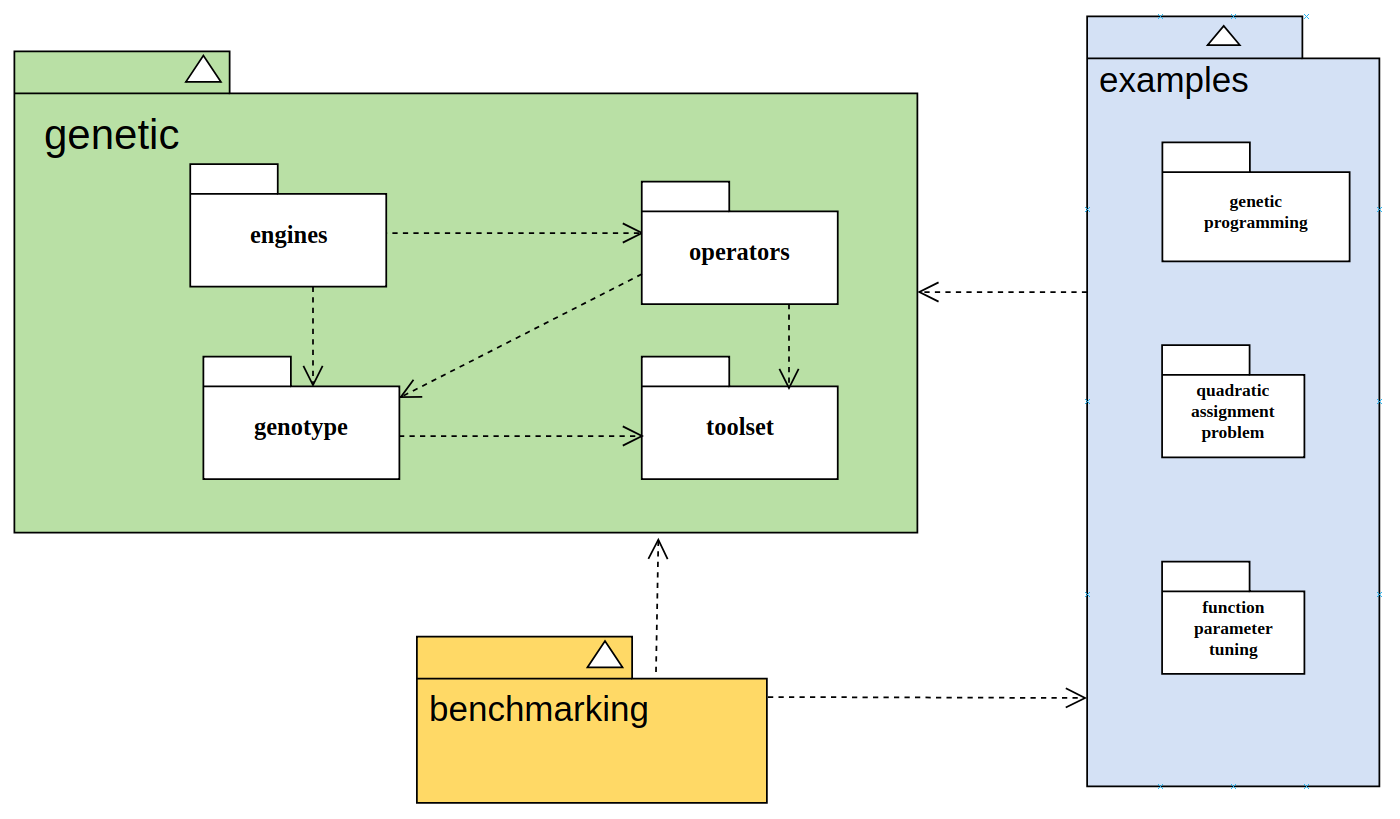
\includegraphics[width=1.\textwidth]{img/diagrams/alleles-top-packages}
\caption{Packages and their source dependencies}\label{diag:packages}
\end{figure}

\textit{genotype} package contains classes, which correspond to the information used to describe behavior of an individual. This is achieved using 4 type classes: \textit{Fitness, Join, Modification} and \textit{Scheme}. This subpackage also contains \textit{CachedFitness} class, which is a wrapper around provided fitness function, with additional caching behavior \ref{diag:genotype-classes}. 

\begin{figure}[h]
\centering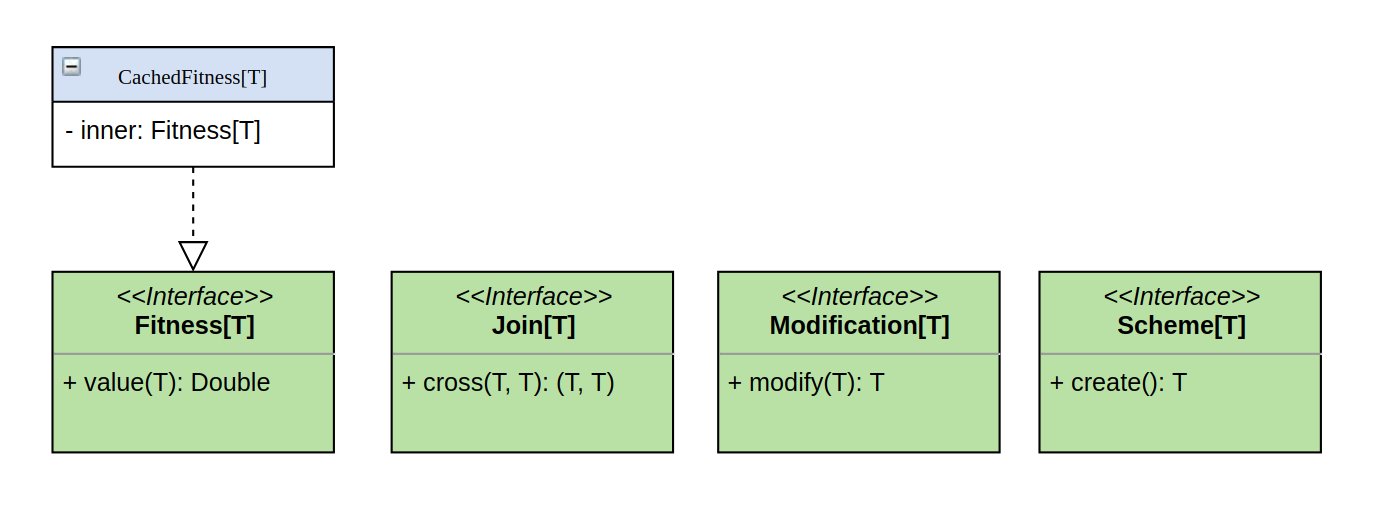
\includegraphics[width=1.\textwidth]{img/diagrams/alleles-genotype}
\caption{Type classes used to describe an individual}\label{diag:genotype-classes}
\end{figure}.

\textit{engines} package contains the heavy part of genetic algorithm implementation. Here one may find EvolutionEnvironment class and its concrete implementations. Every child class (parallel implementation) is placed in its specific subpage, so users have to import only the part, which they are interested in or everything, if this is desired. This approach may be seen in project structure \ref{diag:project-structure}, where the interfaces, which are communicating between each other are placed at the top of the package and different variants of their implementation are placed into specific subpackage, which later is important for user needs.

\smallskip\textit{This satisfies predefined non-functional requirement \ref{nfreq:modul}}

\begin{figure}
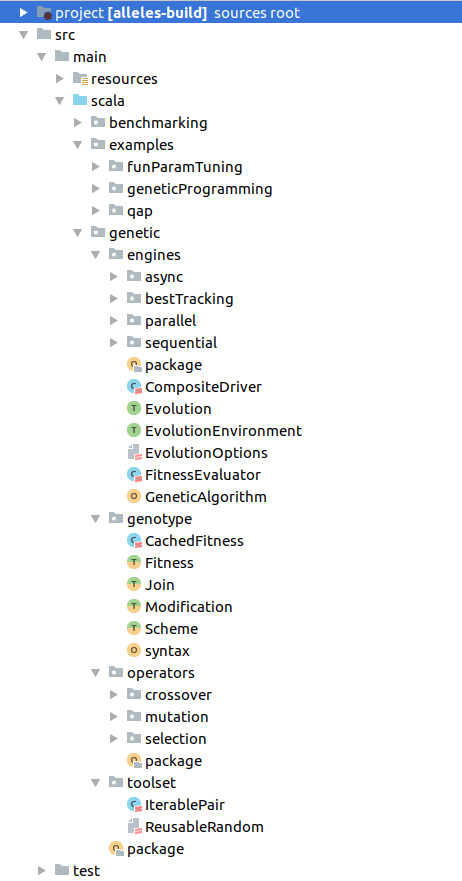
\includegraphics[width=.7\textwidth]{img/diagrams/alleles-project-structure}
\caption{Expanded project structure}\label{diag:project-structure}
\end{figure}

\medbreak
The way in which parts of \textit{engines} package are related to each other may be observed in \textit{genetic} class diagram\ref{diag:genetic-classes}

\begin{figure}
\centering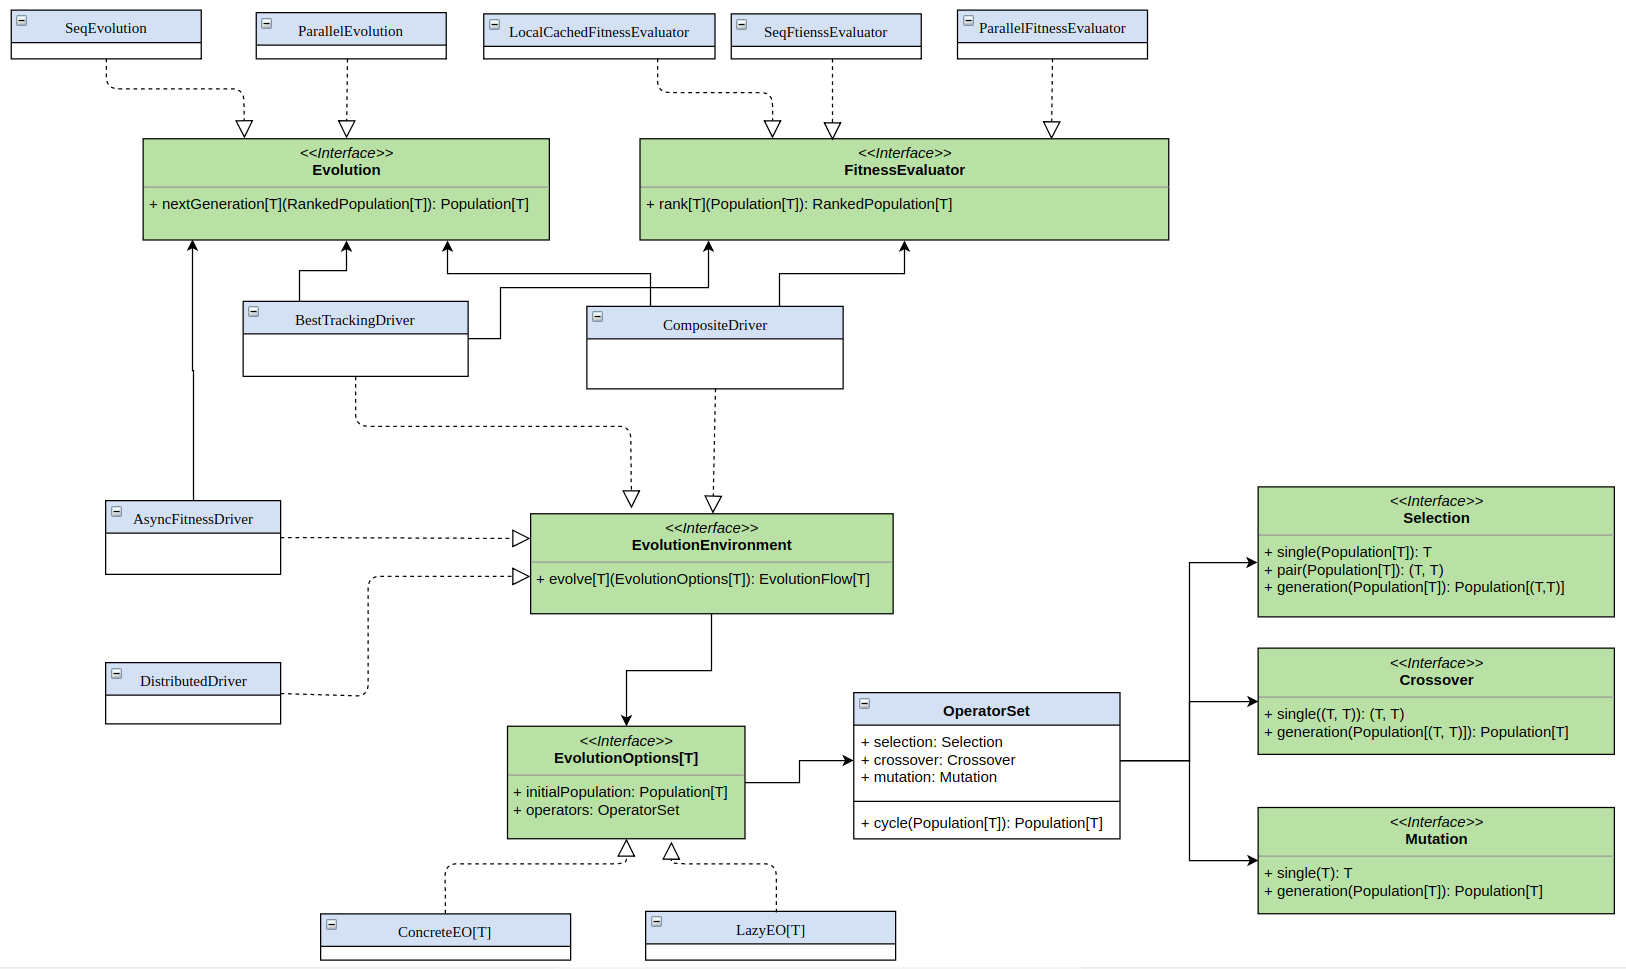
\includegraphics[width=1.\textwidth]{img/diagrams/alleles-genetic-class}
\caption{Classes diagram from \textit{genetic} package}\label{diag:genetic-classes}
\end{figure}